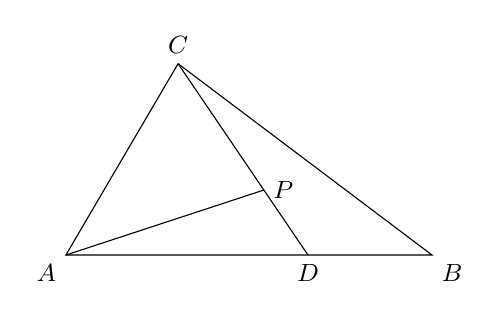
\begin{tikzpicture}[scale=.75, every node/.style={font=\small}]
  \coordinate (A) at (0,0); \coordinate (B) at (6.20,0);
  \coordinate (C) at (1.90,3.24); \coordinate (D) at (4.10,0);
  \coordinate (P) at (3.35,1.10);
  \draw (A)--(B)--(C)--cycle; \draw (C)--(D); \draw (A)--(P);
  \node[below left] at (A) {$A$};
  \node[below right] at (B) {$B$};
  \node[above] at (C) {$C$};
  \node[below] at (D) {$D$};
  \node[right] at (P) {$P$};
\end{tikzpicture}
